\chapter{Desenvolvimento}

Deve-se inserir texto entre as seções.

\section{Exposição Do Tema Ou Matéria}

É a parte principal e mais extensa do trabalho. Deve apresentar a fundamentação teórica, a metodologia, os resultados e a discussão. Divide-se em seções e subseções conforme a NBR6024~\cite{abnt6024}. 
Quanto à sua estrutura e projeto gráfico, segue as recomendações da norma para preparação de trabalhos acadêmicos, a NBR14724~\cite{abnt14724}.

\begin{figure}[!ht]
    \centering
    \caption{Elementos do trabalho acadêmico.}   \label{fig:fig1}
    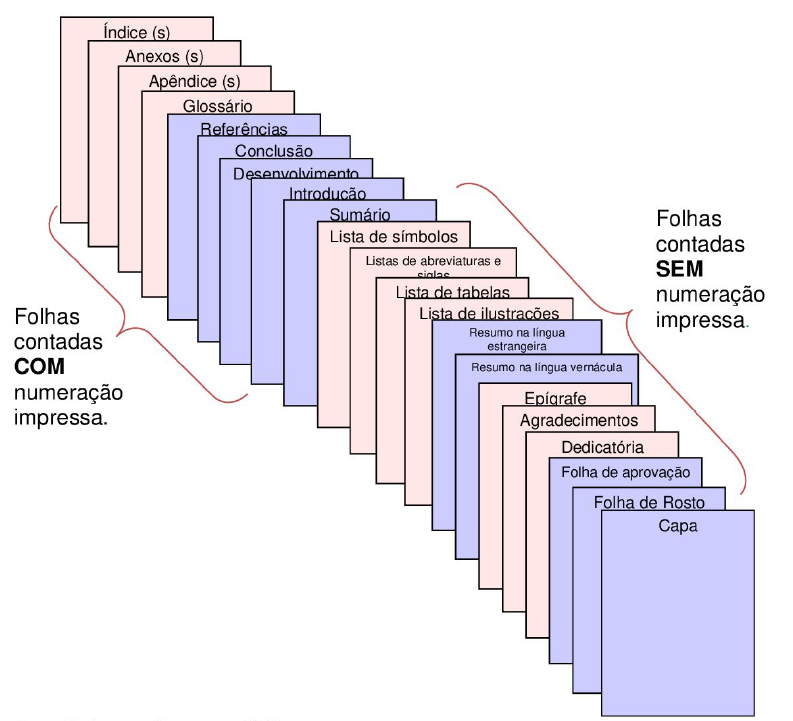
\includegraphics[width = 0.75\textwidth]{images/___fig1.png}
    \legend{\citeauthor{SIBI}}
\end{figure}

\section{Apresentação Gráfica Do Trabalho}
As orientações abaixo se referem a: trabalho de conclusão, monografias, dissertações e teses. Em alguns casos, são adequadas para uso na elaboração de relatórios de estágio, artigos e/ou \textit{paper} elaborados para entrega no IFC.


\subsection{Formato (tipo de papel, tamanho da fonte, margens)}


Apresentação gráfica de uma produção acadêmica a ser entregue na versão digital:

\begin{enumerate}[label=\alph*)]
   \item digitar o texto na cor preta. Cores somente em ilustrações como por exemplo: gráficos;
    \item  utilizar fonte tamanho 12 para o texto;
    \item  utilizar fonte tamanho 10 para citações longas, notas de rodapé, fontes (identificação) das ilustrações e tabelas e paginação;
    \item  optar por fontes arredondadas (\textit{Times New Roman} ou \textit{Arial}); 
    \item  margens:  superior de 3 cm;  inferior de 2 cm;  esquerda de 3 cm; direita de 2 cm.
    \item  inserir recuo de 2 cm, na primeira linha do parágrafo, a partir da margem esquerda;
    \item  inserir recuo de 4 cm, a partir da margem esquerda, na citação longa (com mais de três linhas);
    \item  digitar a nota de rodapé dentro das margens indicadas, devendo esta ficar separada do texto por um traço de 5 cm a partir da margem esquerda (ver seção 10);
    \item  apresentar o texto sobre a “natureza do trabalho” localizado  na folha de rosto e na folha de aprovação, a partir do meio da mancha gráfica para a margem direita (Figuras 12 e 15).
\end{enumerate}


Caso a produção acadêmica também seja entregue no formato impresso, observar os seguintes requisitos adicionais:

\begin{enumerate}[label=\alph*)]
    \item utilizar papel branco ou reciclado, formato A4 (21,0 $\times$ 29,7 cm);
    \item utilizar o anverso da folha para os elementos pré-textuais;
    \item poderá ser utilizado o anverso e verso da folha para impressão dos elementos textuais e pós-textuais;
    \item adotar as margens:
\begin{table}[h!]
\centering
\begin{tabular}{|l|l|} 
\hline
\begin{tabular}[c]{@{}l@{}}- para o anverso da folha:\\-superior de 3 cm,\\-inferior de 2 cm,\\-esquerda de 3 cm,\\-direita de 2 cm.\end{tabular} & \begin{tabular}[c]{@{}l@{}}- para o verso:\\	-superior de 3 cm,\\	-inferior de 2 cm,\\-esquerda de 2 cm,\\	-direita de 3 cm.\end{tabular}  \\
\hline
\end{tabular}
\end{table}
\end{enumerate}


\subsection{Espaçamento}
O espaçamento que você deve adotar na formatação é:
\begin{enumerate}[label=\alph*)]
\item  espaço 1,5:
\begin{itemize}
\item[-] todo o texto;
\end{itemize}
\item um espaço de 1,5:
\begin{itemize}
\item[-] separa o texto da citação longa;
\item[-] separa cada título das seções e subseções do texto que os precede e que os sucede;
\end{itemize}
\item espaço simples para:
\begin{itemize}
\item[-] citações longas;
\item[-] notas de rodapé;
\item[-] referências;
\item[-] legenda e fonte das ilustrações e tabelas;
\item[-] natureza do trabalho;
\end{itemize}
\item um espaço simples:
\begin{itemize} 
\item[--] entre uma referência e outra, na lista de referências ao final do trabalho.
\end{itemize}
\end{enumerate}



\subsection{Indicativo de seção e numeração progressiva}
Seção é a divisão do TA, aplicada somente aos elementos textuais, que visa expor, numa sequência lógica, o relacionamento da matéria e permitir a sua localização. De acordo com a NBR 6024 \cite{abnt6024}, as seções também podem ser subdividas em subseções.
A seção primária é a principal divisão do texto do TA, que sempre deverá ser grafada em números inteiros a partir do 1, alinhados à esquerda por um espaço de caractere, e iniciar em página distinta e ímpar (anverso). As demais são chamadas de subseções e/ou seções secundária, terciária, quaternária e quinaria. Se for necessário enumerar os diversos assuntos de uma seção que não possua título, esta deve ser subdividida em alíneas. As alíneas são ordenadas alfabeticamente e terminam em ponto e vírgula, exceto a última, que termina em ponto. \textbf{Todas as seções devem conter um texto relacionado a elas e só devem ser subdivididas se houver necessidade de mais duas.}

Exemplo sugerido pelo IFC
\begin{itemize}
\item[] \textbf{1  SEÇÃO PRIMÁRIA (maiúsculas em negrito)}
\item[] 1.1  SEÇÃO SECUNDÁRIA (maiúsculas)
\item[] \textbf{1.1.1   Seção terciária (em negrito com primeira letra maiúscula)}
\item[] \textit{1.1.1.1 Seção quaternária (itálico com primeira letra maiúscula)}
\end{itemize}


\subsection{Paginação}
Para o TA, as páginas pré-textuais devem ser contadas, mas não numeradas. A contagem deve iniciar a partir da folha de rosto. Já a numeração propriamente deve aparecer somente a partir da primeira folha textual, em algarismos arábicos, e ser sequencial até o final do trabalho. 
O número da página deve aparecer no canto superior direito da folha, a 2 cm da borda, ficando o último algarismo a 2 cm da borda direita da folha.
A paginação da(s) referência(s), do(s) anexo(s) e do(s) apêndice(s) deve ser numerada sequencialmente no TA. As páginas que não permitem a inclusão de números também são contadas (mapas, documentos, ilustrações, etc.).
Para trabalhos com mais de um volume, a numeração sequencial das folhas deve ser mantida. Se o trabalho contiver apêndice e anexo, a numeração das páginas deve dar sequência ao texto principal.

\section{Ilustrações}
Independentemente do tipo de ilustração (quadro, desenho, figura, fotografia, mapa, entre outros), a sua identificação aparece na parte superior, precedida da palavra designativa. 
\begin{citacao}
Após a ilustração, na parte inferior, indicar a fonte consultada (elemento obrigatório, mesmo que seja produção do próprio autor), legenda, notas e outras informações necessárias à sua compreensão (se houver). A ilustração deve ser citada no texto e inserida o mais próximo possível do texto a que se refere. \cite[p. 11]{abnt14724}.
\end{citacao}

Um exemplo é apresentado na figura \ref{fig:fig2}:


\begin{figure}[!ht]
    \centering
    \caption{Modelo de gráfico}   \label{fig:fig2}
    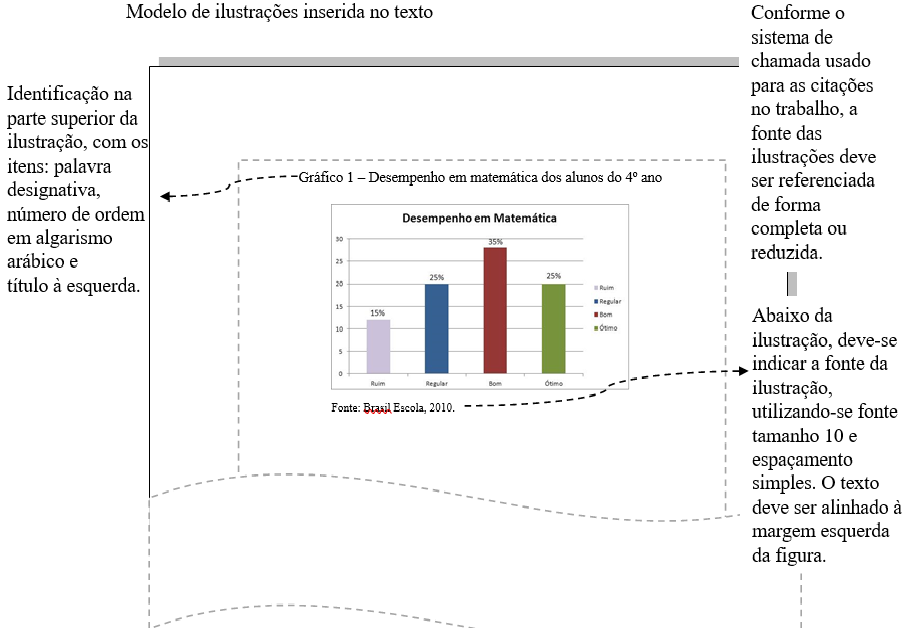
\includegraphics[width = 0.90\textwidth]{images/___fig2.png}
    \legend{\cite{SIBI}}
\end{figure}

\subsection{Equações e fórmulas}
As equações e fórmulas devem ser destacadas no texto para facilitar a leitura.  Para numerá-las, usar algarismos arábicos entre parênteses e alinhados à direita. Pode-se adotar uma entrelinha maior do que a usada no texto \cite{abnt14724}.
Exemplos são apresentados na equações \ref{eq:eq1} e \ref{eq:eq2}.

\begin{equation}
    \dot{x}(KT)\approx \frac{x(k+1)-x(k)}{T}
    \label{eq:eq1}
\end{equation}

\begin{equation}
    \frac{y(k)-y(k-1)}{T}+K\cdot y(t)=K\cdot u(t)
    \label{eq:eq2}
\end{equation}

\subsection{Tabela}

De acordo com Instituto Brasileiro de Geografia e Estatística (1993), tabela é uma forma não discursiva de apresentar informações em que os números representam a informação central. Um exemplo de tabela é encontrado na tabela \ref{tab:tab1}.
\begin{table}[h!]
\centering
\caption{Exemplo de tabela} \label{tab:tab1}
\begin{tabular}{llllllll} 
\hline
\multicolumn{8}{l}{Tabela de exemplo}  \\ 
\hline
aa & 1  & 0  & 0  & 0  & 0  & 0  & 0   \\ 
\hline
bb & zz & 2  & 0  & 0  & 0  & 0  & 0   \\ 
\hline
cc & zz & zz & 3  & 0  & 0  & 0  & 7   \\ 
\hline
dd & zz & zz & zz & 4  & zz & 6  & zz  \\ 
\hline
ee & zz & zz & zz & zz & 5  & zz & zz  \\
\hline
\end{tabular}
\end{table}

\subsection{Código}

\lstinputlisting[
    language=tex,
    caption={Código do sumário.},
    sourcePrefix={Fonte: },
    source={Do autor.},
    label={code:sumario_code}
]{sections/sumario.tex}

